\chapter{Evaluation\label{chap:evaluation}}


%Explain simulation and communication
%Evaluate different models task based
%How where the realisations/ideas tested?
%What were the results of those tests?
%TODO check if this needs to be rewritten, currently only copied from last draft!!!

This chapter describes the different evaluation scenarios that were used to test the trained model 
as well as present the achieved results in each of these scenarios. The presented tests were 
designed to measure the forward models as well as the inverse models performances. The first 
scenario, called the \enquote{Push Task Simulation}, tests the forward models of the different 
concepts, while the second test scenario, the \enquote{Move to target}, tests the inverse models.


\section{Simulation\label{sec:simulation}}

The model is supposed to learn object manipulation through interaction. Instead of on a real robot the model has been developed and tested in a simplified simulation. For this work gazebo \cite{gazebo} V.2.2.3 was used with the physics engine Open Dynamics Engine (ODE) \cite{ode}. This simulation and version were chosen because this thesis was initially planned as a part of a bigger project in the Citec of Bielefeld University where this software was used as well. 

\subsection{World and robot actions \label{sec:environment}}%TODO Check if remained the same

The model was developed with a toy-world consisting of only a sphere, which is 
regarded as actuator, and a rectangular block as can be seen in figure 
\ref{fig:gazeboWorld}.
Since the focus of this work is to learn simple object interactions, the 
possible actions of the robot were limited to moving the actuator freely in two 
dimensions.

\begin{figure} %TODO Check if remained the same
	%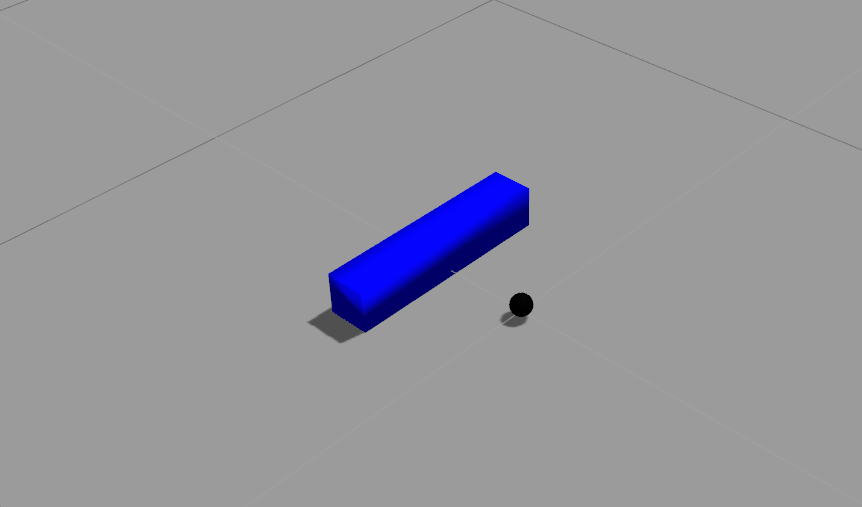
\includegraphics[width=5cm]{images/gazeboWorld.png} %TODO make image
	\caption{Overview of the used world and objects. The sphere represents the 
		robot's actuator and the rectangular block represents the primary object.}
	\label{fig:gazeboWOrld}
\end{figure}


\subsection{Communication}
In order to communicate with the simulation, a plug-in was written, that publishes the properties of all objects using google protobuf \cite{protobuf}. These messages are received and unpacked by a custom python interface that handles the communication with the simulation from the model's side. The plug-in also interprets the commands coming from the interface. A list of all implemented commands can be found in table \ref{tab:commands}

\begin{table}
	\centering
	\begin{tabular}{|c|c|}
		\hline \textbf{Command} & \textbf{Meaning} \\ 
		\hline Move Command & Sets the velocity for the actuator \\ 
		\hline Pause & Pauses the simulation \\
		\hline Unpause & Continues the simulation \\
		\hline Reset & Resets the world to starting configuration \\
		\hline Set Pose & Places a specified object at a certain position \\
		\hline
	\end{tabular} 
	\caption{Overview of all the commands implemented in the model.}
	\label{tab:commands}
\end{table}

\subsection{Sources of noise}
[Describe why there is noise in the data, and where it comes from]
\begin{itemize}
\item Simulation's physics computation not perfectly synchronized %TODO refer to official statement if possible
\item Asynchronous Message communication (not determined when action message is received)
\item Numerical noise from physics computation of (resting-)contacts
\end{itemize}

\section{Push Task Simulation}

This task is designed to test the accuracy of the forward models by decoupling them from the open 
world during successive predictions. 

\subsection{Scenario description}

In this test, the actuator uses a constant action in order to first move towards the block and then push it.
The actuator starts at different starting positions on a line parallel to the block so that the distance along
the action axis always starts at 25cm between the two centers. The block is orientated so that it's main axis
is perpendicular to the action axis.

The model is first trained using the open loop. This means that the model receives all information about the
world at each timestep before making the prediction for the next timestep. This training is done for a set amount
of \enquote{runs}. A run starts when the actuator performs the first action from the starting position and ends after a fixed 
number of iterations or if the actuator travels a predefined distance.
An example starting and end configuration can be seen in figure \ref{fig:pushTaskSim}. 

All starting positions except the first three are chosen randomly, but using the
same seed for all models and configurations. %TODO does not work, not even with the same model just with state3 vs state4... investigate!
The first three are chosen so that the actuator touches the object on the outer left, the outer right side
and directly at the center. This has been done to ensure that the models have seen all general interactions for when they are evaluated with only 3
runs. The random start positions are chosen in such a range, that the actuator can also pass the object without touching it, by sampling starting positions
between -0.35 and 0.35. Another seed is set after the training is done, so that all models are tested on the same starting positions, regardless of
the number of training examples.

The number of iterations used here is 150 when using
the model at 100Hz. During these iterations the actuator moves approximately 75cm. The maximal distance is set to 1m when using the
model with 10Hz. The actual action is the same for both frequencies and is that to 0.5m/s upwards towards the block from the starting
position. 

\begin{figure}
	%TODO make figure !
	
	\caption{TODO Push Task Simulation. The left side shows one exemplary start configuration, while on the right the corresponding end configuration can be seen.
		The darker objects (dark blue and black) represent the actual block and actuator, while the transparent objects symbolize the predicted objects.}
	\label{fig:pushTaskSim}
\end{figure}


\subsection{Evaluation criteria}

This task tries to evaluate the precision of the different models. In order to measure this precision, the predicted actuator position
is compared with the actual actuator position. Since at least the block can also rotate around the third axis, the orientation needs to be
considered as well when measuring the prediction performance. Since it is hard to find a metric that adequately combines point differences with
angular differences, the orientation is indirectly measured. In addition to the center position of each object, two key points are defined that
are located at the edges of the block as can be seen in figure \ref{fig:refPoints}. This way the euclidean distance can be used to measure the
prediction accuracy of both the object's position as well as their orientation. The three distances are then averaged to compute the final difference
score s:

\begin{math}
	s = \frac{1}{3} \sum\limits_{i=1}^{3}||p^{pred}_i-p^{actual}_i||
\end{math}

where $p^{pred}_i, pred^{actual}_i$ represents the i's predicted and actual reference point, including the center, respectively.

These scores are computed at each timestep and accumulated. Furthermore, the final difference, at the last timestep of each run is recorded separately.
The results show the averaged results for the final difference, the accumulated differences and the mean difference over 20 test runs. The mean difference
is computed by dividing the accumulated difference by the number of predictions, the model made in each run, which is equal to the number of iterations-1. For the
first iteration, there has not been a prediction that can be compared yet.

\begin{figure}
	%TODO make image
	
	\caption{TODO Image of the reference points of the block object. The two selected edges, along with the center of the block, make up the three points that are used
		to compare the predicted position with the actual position.}
	\label{fig:refPoints}
\end{figure}

%\subsection{Results}
%%TODO 
%[TODOSome first results of the interaction model. Not perfectly tuned yet, as the DT often selects strange things]
%
%\begin{table}
%	\begin{tabular}{|c|c|c|c|}
%		\hline Model configuration & Final dif & Cum dif & Mean dif \\ 
%		\hline Pairwise AC DT 3 Train & 0.001 & 0.095 & 0.001  \\ 
%		\hline Pairwise AC DT 10 Train & 0.053 & 3.929 & 0.026  \\ 
%		\hline Gate HG HA 3 Train & 0.001 & 0.128 & 0.001 \\
%		\hline Gate HG HA 10 Train ITM $\eta$ 0.0 & 0.001 & 0.127 & 0.001 \\ 
%		\hline Gate HG HA 10 Train ITM $\eta$ 0.1 & 0.001 & 0.122 & 0.001 \\
%		\hline Gate HG HA 10 Train ITM $\eta$ 0.2 & 0.001 & 0.122 & 0.001 \\ 
%		\hline Gate HG HA 10 Train NoAV & 0.001 & 0.135 & 0.001 \\ 
%		\hline Gate HG HA 10 Train NoDyns & 0.001 & 0.130 & 0.001 \\ 
%		\hline 
%	\end{tabular} 
%	\caption{Actuator table showing the results of different realization models. Recorded are the mean differences in the actuator positions and the end of a run, the total accumulated difference and the mean difference over a run.}
%\end{table}
%
%\begin{table}
%	\begin{tabular}{|c|c|c|c|}
%		\hline Model configuration & Final dif & Cum dif & Mean dif \\ 
%		\hline Pairwise AC DT 3 Train & 0.209 & 14.051 & 0.094  \\ 
%		\hline Pairwise AC DT 10 Train & 0.142 & 10.841 & 0.073  \\
%		\hline Gate HG HA 3 Train & 0.048 & 3.061 & 0.021 \\ 
%		\hline Gate HG HA 10 Train ITM $\eta$ 0.0 & 0.052 & 3.189 & 0.021 \\ 
%		\hline Gate HG HA 10 Train ITM $\eta$ 0.1 & 0.046 & 2.968 & 0.020 \\ 
%		\hline Gate HG HA 10 Train ITM $\eta$ 0.2 & 0.061 & 3.538 & 0.024 \\ 
%		\hline Gate HG HA 10 Train NoAV & 0.050 & 2.859 & 0.019 \\ 
%		\hline Gate HG HA 10 Train NoDyns & 0.068 & 4.670 & 0.031 \\ 
%		\hline 
%	\end{tabular} 
%	\caption{Block table showing the results of different realization models. Recorded are the mean differences in the block positions and the end of a run, the total accumulated difference and the mean difference over a run.}
%\end{table}

%TODO Also test only interaction prediction performance, by removing all the instances where only the gripper moved!



\section{Move to target}

\subsection{Scenario description}

\subsection{Evaluation criteria}

\subsection{Results}